%% bare_jrnl.tex
%% V1.3
%% 2007/01/11
%% by Michael Shell
%% see http://www.michaelshell.org/
%% for current contact information.
%%
%% This is a skeleton file demonstrating the use of IEEEtran.cls
%% (requires IEEEtran.cls version 1.7 or later) with an IEEE journal paper.
%%
%% Support sites:
%% http://www.michaelshell.org/tex/ieeetran/
%% http://www.ctan.org/tex-archive/macros/latex/contrib/IEEEtran/
%% and
%% http://www.ieee.org/



% *** Authors should verify (and, if needed, correct) their LaTeX system  ***
% *** with the testflow diagnostic prior to trusting their LaTeX platform ***
% *** with production work. IEEE's font choices can trigger bugs that do  ***
% *** not appear when using other class files.                            ***
% The testflow support page is at:
% http://www.michaelshell.org/tex/testflow/


%%*************************************************************************
%% Legal Notice:
%% This code is offered as-is without any warranty either expressed or
%% implied; without even the implied warranty of MERCHANTABILITY or
%% FITNESS FOR A PARTICULAR PURPOSE! 
%% User assumes all risk.
%% In no event shall IEEE or any contributor to this code be liable for
%% any damages or losses, including, but not limited to, incidental,
%% consequential, or any other damages, resulting from the use or misuse
%% of any information contained here.
%%
%% All comments are the opinions of their respective authors and are not
%% necessarily endorsed by the IEEE.
%%
%% This work is distributed under the LaTeX Project Public License (LPPL)
%% ( http://www.latex-project.org/ ) version 1.3, and may be freely used,
%% distributed and modified. A copy of the LPPL, version 1.3, is included
%% in the base LaTeX documentation of all distributions of LaTeX released
%% 2003/12/01 or later.
%% Retain all contribution notices and credits.
%% ** Modified files should be clearly indicated as such, including  **
%% ** renaming them and changing author support contact information. **
%%
%% File list of work: IEEEtran.cls, IEEEtran_HOWTO.pdf, bare_adv.tex,
%%                    bare_conf.tex, bare_jrnl.tex, bare_jrnl_compsoc.tex
%%*************************************************************************

% Note that the a4paper option is mainly intended so that authors in
% countries using A4 can easily print to A4 and see how their papers will
% look in print - the typesetting of the document will not typically be
% affected with changes in paper size (but the bottom and side margins will).
% Use the testflow package mentioned above to verify correct handling of
% both paper sizes by the user's LaTeX system.
%
% Also note that the "draftcls" or "draftclsnofoot", not "draft", option
% should be used if it is desired that the figures are to be displayed in
% draft mode.
%
\documentclass[journal]{IEEEtran}
%
% If IEEEtran.cls has not been installed into the LaTeX system files,
% manually specify the path to it like:
% \documentclass[journal]{../sty/IEEEtran}





% Some very useful LaTeX packages include:
% (uncomment the ones you want to load)


% *** MISC UTILITY PACKAGES ***
%
%\usepackage{ifpdf}
% Heiko Oberdiek's ifpdf.sty is very useful if you need conditional
% compilation based on whether the output is pdf or dvi.
% usage:
% \ifpdf
%   % pdf code
% \else
%   % dvi code
% \fi
% The latest version of ifpdf.sty can be obtained from:
% http://www.ctan.org/tex-archive/macros/latex/contrib/oberdiek/
% Also, note that IEEEtran.cls V1.7 and later provides a builtin
% \ifCLASSINFOpdf conditional that works the same way.
% When switching from latex to pdflatex and vice-versa, the compiler may
% have to be run twice to clear warning/error messages.






% *** CITATION PACKAGES ***
%
%\usepackage{cite}
% cite.sty was written by Donald Arseneau
% V1.6 and later of IEEEtran pre-defines the format of the cite.sty package
% \cite{} output to follow that of IEEE. Loading the cite package will
% result in citation numbers being automatically sorted and properly
% "compressed/ranged". e.g., [1], [9], [2], [7], [5], [6] without using
% cite.sty will become [1], [2], [5]--[7], [9] using cite.sty. cite.sty's
% \cite will automatically add leading space, if needed. Use cite.sty's
% noadjust option (cite.sty V3.8 and later) if you want to turn this off.
% cite.sty is already installed on most LaTeX systems. Be sure and use
% version 4.0 (2003-05-27) and later if using hyperref.sty. cite.sty does
% not currently provide for hyperlinked citations.
% The latest version can be obtained at:
% http://www.ctan.org/tex-archive/macros/latex/contrib/cite/
% The documentation is contained in the cite.sty file itself.






% *** GRAPHICS RELATED PACKAGES ***
%
\ifCLASSINFOpdf
  \usepackage[pdftex]{graphicx}
  % declare the path(s) where your graphic files are
  % \graphicspath{{../pdf/}{../jpeg/}}
  % and their extensions so you won't have to specify these with
  % every instance of \includegraphics
  %\DeclareGraphicsExtensions{.pdf}
  \DeclareGraphicsExtensions{.pdf,.jpeg,.jpg,.png}
\else
  % or other class option (dvipsone, dvipdf, if not using dvips). graphicx
  % will default to the driver specified in the system graphics.cfg if no
  % driver is specified.
  \usepackage[dvips]{graphicx}
  % declare the path(s) where your graphic files are
  % \graphicspath{{../eps/}}
  % and their extensions so you won't have to specify these with
  % every instance of \includegraphics
  \DeclareGraphicsExtensions{.eps}
\fi
% graphicx was written by David Carlisle and Sebastian Rahtz. It is
% required if you want graphics, photos, etc. graphicx.sty is already
% installed on most LaTeX systems. The latest version and documentation can
% be obtained at: 
% http://www.ctan.org/tex-archive/macros/latex/required/graphics/
% Another good source of documentation is "Using Imported Graphics in
% LaTeX2e" by Keith Reckdahl which can be found as epslatex.ps or
% epslatex.pdf at: http://www.ctan.org/tex-archive/info/
%
% latex, and pdflatex in dvi mode, support graphics in encapsulated
% postscript (.eps) format. pdflatex in pdf mode supports graphics
% in .pdf, .jpeg, .png and .mps (metapost) formats. Users should ensure
% that all non-photo figures use a vector format (.eps, .pdf, .mps) and
% not a bitmapped formats (.jpeg, .png). IEEE frowns on bitmapped formats
% which can result in "jaggedy"/blurry rendering of lines and letters as
% well as large increases in file sizes.
%
% You can find documentation about the pdfTeX application at:
% http://www.tug.org/applications/pdftex





% *** MATH PACKAGES ***
%
%\usepackage[cmex10]{amsmath}
% A popular package from the American Mathematical Society that provides
% many useful and powerful commands for dealing with mathematics. If using
% it, be sure to load this package with the cmex10 option to ensure that
% only type 1 fonts will utilized at all point sizes. Without this option,
% it is possible that some math symbols, particularly those within
% footnotes, will be rendered in bitmap form which will result in a
% document that can not be IEEE Xplore compliant!
%
% Also, note that the amsmath package sets \interdisplaylinepenalty to 10000
% thus preventing page breaks from occurring within multiline equations. Use:
%\interdisplaylinepenalty=2500
% after loading amsmath to restore such page breaks as IEEEtran.cls normally
% does. amsmath.sty is already installed on most LaTeX systems. The latest
% version and documentation can be obtained at:
% http://www.ctan.org/tex-archive/macros/latex/required/amslatex/math/





% *** SPECIALIZED LIST PACKAGES ***
%
%\usepackage{algorithmic}
% algorithmic.sty was written by Peter Williams and Rogerio Brito.
% This package provides an algorithmic environment fo describing algorithms.
% You can use the algorithmic environment in-text or within a figure
% environment to provide for a floating algorithm. Do NOT use the algorithm
% floating environment provided by algorithm.sty (by the same authors) or
% algorithm2e.sty (by Christophe Fiorio) as IEEE does not use dedicated
% algorithm float types and packages that provide these will not provide
% correct IEEE style captions. The latest version and documentation of
% algorithmic.sty can be obtained at:
% http://www.ctan.org/tex-archive/macros/latex/contrib/algorithms/
% There is also a support site at:
% http://algorithms.berlios.de/index.html
% Also of interest may be the (relatively newer and more customizable)
% algorithmicx.sty package by Szasz Janos:
% http://www.ctan.org/tex-archive/macros/latex/contrib/algorithmicx/




% *** ALIGNMENT PACKAGES ***
%
%\usepackage{array}
% Frank Mittelbach's and David Carlisle's array.sty patches and improves
% the standard LaTeX2e array and tabular environments to provide better
% appearance and additional user controls. As the default LaTeX2e table
% generation code is lacking to the point of almost being broken with
% respect to the quality of the end results, all users are strongly
% advised to use an enhanced (at the very least that provided by array.sty)
% set of table tools. array.sty is already installed on most systems. The
% latest version and documentation can be obtained at:
% http://www.ctan.org/tex-archive/macros/latex/required/tools/


%\usepackage{mdwmath}
%\usepackage{mdwtab}
% Also highly recommended is Mark Wooding's extremely powerful MDW tools,
% especially mdwmath.sty and mdwtab.sty which are used to format equations
% and tables, respectively. The MDWtools set is already installed on most
% LaTeX systems. The lastest version and documentation is available at:
% http://www.ctan.org/tex-archive/macros/latex/contrib/mdwtools/


% IEEEtran contains the IEEEeqnarray family of commands that can be used to
% generate multiline equations as well as matrices, tables, etc., of high
% quality.


%\usepackage{eqparbox}
% Also of notable interest is Scott Pakin's eqparbox package for creating
% (automatically sized) equal width boxes - aka "natural width parboxes".
% Available at:
% http://www.ctan.org/tex-archive/macros/latex/contrib/eqparbox/





% *** SUBFIGURE PACKAGES ***
%\usepackage[tight,footnotesize]{subfigure}
% subfigure.sty was written by Steven Douglas Cochran. This package makes it
% easy to put subfigures in your figures. e.g., "Figure 1a and 1b". For IEEE
% work, it is a good idea to load it with the tight package option to reduce
% the amount of white space around the subfigures. subfigure.sty is already
% installed on most LaTeX systems. The latest version and documentation can
% be obtained at:
% http://www.ctan.org/tex-archive/obsolete/macros/latex/contrib/subfigure/
% subfigure.sty has been superceeded by subfig.sty.



%\usepackage[caption=false]{caption}
%\usepackage[font=footnotesize]{subfig}
% subfig.sty, also written by Steven Douglas Cochran, is the modern
% replacement for subfigure.sty. However, subfig.sty requires and
% automatically loads Axel Sommerfeldt's caption.sty which will override
% IEEEtran.cls handling of captions and this will result in nonIEEE style
% figure/table captions. To prevent this problem, be sure and preload
% caption.sty with its "caption=false" package option. This is will preserve
% IEEEtran.cls handing of captions. Version 1.3 (2005/06/28) and later 
% (recommended due to many improvements over 1.2) of subfig.sty supports
% the caption=false option directly:
%\usepackage[caption=false,font=footnotesize]{subfig}
%
% The latest version and documentation can be obtained at:
% http://www.ctan.org/tex-archive/macros/latex/contrib/subfig/
% The latest version and documentation of caption.sty can be obtained at:
% http://www.ctan.org/tex-archive/macros/latex/contrib/caption/




% *** FLOAT PACKAGES ***
%
%\usepackage{fixltx2e}
% fixltx2e, the successor to the earlier fix2col.sty, was written by
% Frank Mittelbach and David Carlisle. This package corrects a few problems
% in the LaTeX2e kernel, the most notable of which is that in current
% LaTeX2e releases, the ordering of single and double column floats is not
% guaranteed to be preserved. Thus, an unpatched LaTeX2e can allow a
% single column figure to be placed prior to an earlier double column
% figure. The latest version and documentation can be found at:
% http://www.ctan.org/tex-archive/macros/latex/base/



%\usepackage{stfloats}
% stfloats.sty was written by Sigitas Tolusis. This package gives LaTeX2e
% the ability to do double column floats at the bottom of the page as well
% as the top. (e.g., "\begin{figure*}[!b]" is not normally possible in
% LaTeX2e). It also provides a command:
%\fnbelowfloat
% to enable the placement of footnotes below bottom floats (the standard
% LaTeX2e kernel puts them above bottom floats). This is an invasive package
% which rewrites many portions of the LaTeX2e float routines. It may not work
% with other packages that modify the LaTeX2e float routines. The latest
% version and documentation can be obtained at:
% http://www.ctan.org/tex-archive/macros/latex/contrib/sttools/
% Documentation is contained in the stfloats.sty comments as well as in the
% presfull.pdf file. Do not use the stfloats baselinefloat ability as IEEE
% does not allow \baselineskip to stretch. Authors submitting work to the
% IEEE should note that IEEE rarely uses double column equations and
% that authors should try to avoid such use. Do not be tempted to use the
% cuted.sty or midfloat.sty packages (also by Sigitas Tolusis) as IEEE does
% not format its papers in such ways.


%\ifCLASSOPTIONcaptionsoff
%  \usepackage[nomarkers]{endfloat}
% \let\MYoriglatexcaption\caption
% \renewcommand{\caption}[2][\relax]{\MYoriglatexcaption[#2]{#2}}
%\fi
% endfloat.sty was written by James Darrell McCauley and Jeff Goldberg.
% This package may be useful when used in conjunction with IEEEtran.cls'
% captionsoff option. Some IEEE journals/societies require that submissions
% have lists of figures/tables at the end of the paper and that
% figures/tables without any captions are placed on a page by themselves at
% the end of the document. If needed, the draftcls IEEEtran class option or
% \CLASSINPUTbaselinestretch interface can be used to increase the line
% spacing as well. Be sure and use the nomarkers option of endfloat to
% prevent endfloat from "marking" where the figures would have been placed
% in the text. The two hack lines of code above are a slight modification of
% that suggested by in the endfloat docs (section 8.3.1) to ensure that
% the full captions always appear in the list of figures/tables - even if
% the user used the short optional argument of \caption[]{}.
% IEEE papers do not typically make use of \caption[]'s optional argument,
% so this should not be an issue. A similar trick can be used to disable
% captions of packages such as subfig.sty that lack options to turn off
% the subcaptions:
% For subfig.sty:
% \let\MYorigsubfloat\subfloat
% \renewcommand{\subfloat}[2][\relax]{\MYorigsubfloat[]{#2}}
% For subfigure.sty:
% \let\MYorigsubfigure\subfigure
% \renewcommand{\subfigure}[2][\relax]{\MYorigsubfigure[]{#2}}
% However, the above trick will not work if both optional arguments of
% the \subfloat/subfig command are used. Furthermore, there needs to be a
% description of each subfigure *somewhere* and endfloat does not add
% subfigure captions to its list of figures. Thus, the best approach is to
% avoid the use of subfigure captions (many IEEE journals avoid them anyway)
% and instead reference/explain all the subfigures within the main caption.
% The latest version of endfloat.sty and its documentation can obtained at:
% http://www.ctan.org/tex-archive/macros/latex/contrib/endfloat/
%
% The IEEEtran \ifCLASSOPTIONcaptionsoff conditional can also be used
% later in the document, say, to conditionally put the References on a 
% page by themselves.





% *** PDF, URL AND HYPERLINK PACKAGES ***
%
%\usepackage{url}
% url.sty was written by Donald Arseneau. It provides better support for
% handling and breaking URLs. url.sty is already installed on most LaTeX
% systems. The latest version can be obtained at:
% http://www.ctan.org/tex-archive/macros/latex/contrib/misc/
% Read the url.sty source comments for usage information. Basically,
% \url{my_url_here}.


\usepackage{eurosym}



% *** Do not adjust lengths that control margins, column widths, etc. ***
% *** Do not use packages that alter fonts (such as pslatex).         ***
% There should be no need to do such things with IEEEtran.cls V1.6 and later.
% (Unless specifically asked to do so by the journal or conference you plan
% to submit to, of course. )


% correct bad hyphenation here
\hyphenation{op-tical net-works semi-conduc-tor}


\begin{document}
%
% paper title
% can use linebreaks \\ within to get better formatting as desired
\title{Overview of the LOFAR signal processing architecture}
%
%
% author names and IEEE memberships
% note positions of commas and nonbreaking spaces ( ~ ) LaTeX will not break
% a structure at a ~ so this keeps an author's name from being broken across
% two lines.
% use \thanks{} to gain access to the first footnote area
% a separate \thanks must be used for each paragraph as LaTeX2e's \thanks
% was not built to handle multiple paragraphs
%

\author{Andr\'{e} W. Gunst,
        Ronald Nijboer,
        and~John W. Romein% <-this % stops a space
\thanks{A. Gunst, R. Nijboer, and J.W. Romein are with ASTRON, Dwingeloo, 
The Netherlands, www.astron.nl
}% <-this % stops a space
\thanks{Manuscript received January 31, 2008; revised .}}

% note the % following the last \IEEEmembership and also \thanks - 
% these prevent an unwanted space from occurring between the last author name
% and the end of the author line. i.e., if you had this:
% 
% \author{....lastname \thanks{...} \thanks{...} }
%                     ^------------^------------^----Do not want these spaces!
%
% a space would be appended to the last name and could cause every name on that
% line to be shifted left slightly. This is one of those "LaTeX things". For
% instance, "\textbf{A} \textbf{B}" will typeset as "A B" not "AB". To get
% "AB" then you have to do: "\textbf{A}\textbf{B}"
% \thanks is no different in this regard, so shield the last } of each \thanks
% that ends a line with a % and do not let a space in before the next \thanks.
% Spaces after \IEEEmembership other than the last one are OK (and needed) as
% you are supposed to have spaces between the names. For what it is worth,
% this is a minor point as most people would not even notice if the said evil
% space somehow managed to creep in.



% The paper headers
\markboth{IEEE Journal of Selected Topics in Signal Processing,~Vol.~X, No.~Y, January~2008}%
{Gunst \MakeLowercase{\textit{et al.}}: Overview of the LOFAR signal processing architecture}
% The only time the second header will appear is for the odd numbered pages
% after the title page when using the twoside option.
% 
% *** Note that you probably will NOT want to include the author's ***
% *** name in the headers of peer review papers.                   ***
% You can use \ifCLASSOPTIONpeerreview for conditional compilation here if
% you desire.




% If you want to put a publisher's ID mark on the page you can do it like
% this:
%\IEEEpubid{0000--0000/00\$00.00~\copyright~2007 IEEE}
% Remember, if you use this you must call \IEEEpubidadjcol in the second
% column for its text to clear the IEEEpubid mark.



% use for special paper notices
%\IEEEspecialpapernotice{(Invited Paper)}


\newcommand{\fixme}[1]{{\bf\em #1}}


% make the title area
\maketitle


\begin{abstract}
%\boldmath
LOFAR is the first of a new generation of phased-array radio telescopes,
that combines the signals from many thousands of simple, omni-directional
antennas, rather than from expensive dishes.
Its revolutionary design and unprecedented size enables observations in the
hardly-explored 10--250~MHz frequency range, and allows the study of
a vast amount of new science cases.

This paper describes the LOFAR signal processing chain from the stations,
where the signals are received to the Central 
Processors. The Central processing is split in real-time correlation and 
off-line calibration and imaging.
\end{abstract}
% IEEEtran.cls defaults to using nonbold math in the Abstract.
% This preserves the distinction between vectors and scalars. However,
% if the journal you are submitting to favors bold math in the abstract,
% then you can use LaTeX's standard command \boldmath at the very start
% of the abstract to achieve this. Many IEEE journals frown on math
% in the abstract anyway.

% Note that keywords are not normally used for peerreview papers.
%\begin{IEEEkeywords}
%IEEEtran, journal, \LaTeX, paper, template.
%\end{IEEEkeywords}






% For peer review papers, you can put extra information on the cover
% page as needed:
% \ifCLASSOPTIONpeerreview
% \begin{center} \bfseries EDICS Category: 3-BBND \end{center}
% \fi
%
% For peerreview papers, this IEEEtran command inserts a page break and
% creates the second title. It will be ignored for other modes.
\IEEEpeerreviewmaketitle



\section{Introduction}
% The very first letter is a 2 line initial drop letter followed
% by the rest of the first word in caps.
% 
% form to use if the first word consists of a single letter:
% \IEEEPARstart{A}{demo} file is ....
% 
% form to use if you need the single drop letter followed by
% normal text (unknown if ever used by IEEE):
% \IEEEPARstart{A}{}demo file is ....
% 
% Some journals put the first two words in caps:
% \IEEEPARstart{T}{his demo} file is ....
% 
% Here we have the typical use of a "T" for an initial drop letter
% and "HIS" in caps to complete the first word.
%\IEEEPARstart{T}{his} demo file is intended to serve as a ``starter file''
%for IEEE journal papers produced under \LaTeX\ using
%IEEEtran.cls version 1.7 and later.
% You must have at least 2 lines in the paragraph with the drop letter
% (should never be an issue)
%I wish you the best of success.

\IEEEPARstart{I}{n} the Netherlands a LO(w) Frequency ARray (LOFAR) is developed for radio astronomy optimized for the frequency band from 30--240 MHz. LOFAR is the first large scale radio telescope based fully on the phased array technique. This prevents the use of moving large constructions and enables multi-beaming. The total collecting area of LOFAR is achieved by many small dipoles which are grouped in stations to reduce the data rate to an acceptable level. The main reduction is achieved by selecting only a part of the sky by using the phased array technique. The number of stations installed in the Netherlands will be at least 36. Half of the number of stations will be core stations and the other half remote stations. The main difference between them is that the core stations can be split up in two independent arrays delivering the two fold of the remote station bandwidth.
\begin{itemize}
\item For the low frequencies involved in LOFAR traditional telescopes would be very large and hence costly
\item Pointing can be done electronically, without using moveable parts and hence saving on maintenance costs
\item Pointing is enabled in multiple directions at the same time
\item  Operational flexibility is enhanced significantly (e.g. rapid switching between observations is possible
\end{itemize}


Since the concept of LOFAR is so different compared with the traditional radio telescopes, the astronomical science that can be done with it is completely different as well. Despite the new concept the processing steps of a radio telescope remain the same. The general data path for an aperture synthesis array is depicted in Figure~\ref{fig:concept}.

\begin{figure}
\begin{center}
\includegraphics[width=53mm]{telescope_overview.eps}
\end{center}
\caption{LOFAR remote station architecture.}
\label{fig:concept}
\end{figure}

In LOFAR, the detector is composed of multiple sensors. Since these sensors convert electromagnetic radiation into electronic signals, the sensors are further referred to as antennas. Ideally, the number of detectors equals the number of antennas to accommodate all sky imaging. However, cost of data transport and processing power limits the number of detectors which can be afforded for a feasible design with a reasonable price. The analog processing shown in Figure~\ref{fig:concept} covers the (low noise) amplification, filtering, analog signal transport and further signal conditioning functions before the signal is converted into the digital domain (Analog/Digital (A/D) conversion block). From there, the signals are digitally conditioned before entering the correlator. Typical operations in LOFAR digital processing are frequency selection, beam forming, delay tracking and fringe stopping. In the correlator, all signals are correlated with each other to form the cross correlation matrix. Furthermore, the correlation results are calibrated for instrumental and environmental effects. Additionally, known sources are subtracted to enhance the dynamic range. Another post processing task is to transform the correlation products into an image.

For LOFAR, the sensors should be distributed over a large area to achieve an angular resolution of arcsec accuracy with an acceptable UV coverage. All data coming from the sensors should come together in the correlator. So, on the one hand the instrument should be distributed over a large area, while on the other hand all data should come together in a central location. To balance the hardware and operational costs between (1) the equipment in the field, (2) the transport network and (3) the volume of the central systems, multiple antennas (96) are grouped in so called stations. Within such a station the information of all individual antennas is weighted and summed. Such an array of antennas is often called a phased array. By using this technique a spatial selection on the sky is made, which reduces the instantaneous Field Of View (FOV) of each station. The main reason for this is to reduce the total data stream to the correlator.

For at least two Key Science Projects (KSPs) a larger FOV is required in the core of the instrument (2 km in diameter) than at extended ranges. Since there is only a limited distance to bridge from the core to the central processing location, more beams, requiring more bandwidth, can be generated in the core. Hence, in LOFAR two types of stations are distinguished: the remote stations and the core stations. 
The main difference between them is that the core stations can be split up in two independent arrays delivering the two fold of the remote station bandwidth.

The number of stations installed in the Netherlands will be at least 36. Half of the number of stations will be core stations and the other half remote stations. 

All data of the stations is transported to one central place via a Wide Area Network (WAN) and using owned and leased light paths. In Groningen all station data is processed. The processing is done by off the shelf hardware, varying from a supercomputer to clusters of computers. The processing done will accomodate for several pipelines, amongst them are pipelines for imaging modes for applications like the Epoch Of Reionization (EOR), surveys and transients and tied-array beamforming for applications like pulsars. However, also more sophisticated processing will be done to enable various energy cosmic ray mode pipelines of different intensities. 

The heart of LOFAR will be installed in the Northern part of the Netherlands. The maximum baseline of LOFAR including only the Dutch stations is about 100 km. Since, also other European institutes show interest and are building LOFAR stations the maximal baseline of LOFAR will be extended, possible to 1000~km.  

%\hfill mds
 
%\hfill January 11, 2007

%\subsection{Subsection Heading Here}
%Subsection text here.

% needed in second column of first page if using \IEEEpubid
%\IEEEpubidadjcol

%\subsubsection{Subsubsection Heading Here}
%Subsubsection text here.


% An example of a floating figure using the graphicx package.
% Note that \label must occur AFTER (or within) \caption.
% For figures, \caption should occur after the \includegraphics.
% Note that IEEEtran v1.7 and later has special internal code that
% is designed to preserve the operation of \label within \caption
% even when the captionsoff option is in effect. However, because
% of issues like this, it may be the safest practice to put all your
% \label just after \caption rather than within \caption{}.
%
% Reminder: the "draftcls" or "draftclsnofoot", not "draft", class
% option should be used if it is desired that the figures are to be
% displayed while in draft mode.
%
%\begin{figure}[!t]
%\centering
%\includegraphics[width=2.5in]{myfigure}
% where an .eps filename suffix will be assumed under latex, 
% and a .pdf suffix will be assumed for pdflatex; or what has been declared
% via \DeclareGraphicsExtensions.
%\caption{Simulation Results}
%\label{fig_sim}
%\end{figure}

% Note that IEEE typically puts floats only at the top, even when this
% results in a large percentage of a column being occupied by floats.


% An example of a double column floating figure using two subfigures.
% (The subfig.sty package must be loaded for this to work.)
% The subfigure \label commands are set within each subfloat command, the
% \label for the overall figure must come after \caption.
% \hfil must be used as a separator to get equal spacing.
% The subfigure.sty package works much the same way, except \subfigure is
% used instead of \subfloat.
%
%\begin{figure*}[!t]
%\centerline{\subfloat[Case I]\includegraphics[width=2.5in]{subfigcase1}%
%\label{fig_first_case}}
%\hfil
%\subfloat[Case II]{\includegraphics[width=2.5in]{subfigcase2}%
%\label{fig_second_case}}}
%\caption{Simulation results}
%\label{fig_sim}
%\end{figure*}
%
% Note that often IEEE papers with subfigures do not employ subfigure
% captions (using the optional argument to \subfloat), but instead will
% reference/describe all of them (a), (b), etc., within the main caption.


% An example of a floating table. Note that, for IEEE style tables, the 
% \caption command should come BEFORE the table. Table text will default to
% \footnotesize as IEEE normally uses this smaller font for tables.
% The \label must come after \caption as always.
%
%\begin{table}[!t]
%% increase table row spacing, adjust to taste
%\renewcommand{\arraystretch}{1.3}
% if using array.sty, it might be a good idea to tweak the value of
% \extrarowheight as needed to properly center the text within the cells
%\caption{An Example of a Table}
%\label{table_example}
%\centering
%% Some packages, such as MDW tools, offer better commands for making tables
%% than the plain LaTeX2e tabular which is used here.
%\begin{tabular}{|c||c|}
%\hline
%One & Two\\
%\hline
%Three & Four\\
%\hline
%\end{tabular}
%\end{table}


% Note that IEEE does not put floats in the very first column - or typically
% anywhere on the first page for that matter. Also, in-text middle ("here")
% positioning is not used. Most IEEE journals use top floats exclusively.
% Note that, LaTeX2e, unlike IEEE journals, places footnotes above bottom
% floats. This can be corrected via the \fnbelowfloat command of the
% stfloats package.

\section{Station processing}

In the LOFAR stations the electromagnetic signals of interest are received by multiple dipoles to achieve the sensitivity requirements. At station levels all of these dipoles are combined by beam forming to reduce the data rate and processing required. The main station architecture is depicted in Figure~\ref{fig:stationarch}. Each subsystem will be discussed in the next subsections.

\begin{figure}
\begin{center}
\includegraphics[width=53mm]{stationoverview.eps}
\end{center}
\caption{LOFAR remote station architecture.}
\label{fig:stationarch}
\end{figure}

\subsection{Antennas}

The operating frequency range of LOFAR is from 10 MHz to 240 MHz, while the antennas should be optimized for the range 30--80 MHz and 120--240 MHz. Since, the optimized bandwidth of the operating frequency range spans 8 octaves at least two types of antennas are necessary in order to fulfill the sensitivity requirements. Therefore, two types of antennas are developed: the Low Band Antenna (LBA) and the High Band Antenna (HBA). To accommodate science below 30 MHz an extra provision is made for a third antenna, also referred to as the Low Band Low (LBL) antenna. In that context the LBA is also referred to as Low Band High (LBH) antenna. All antennas are designed for two polarizations.

In total 48 LBL, 48 LBH and 48 HBA tiles will be installed in a station. The HBA is organized in tiles, wherein 16 antenne elements are combined via analog beamforming to yield a comparable effective area for both the low band and high band antennas. Analog beamforming for the HBAs is used to combine the 16 antenna elements at tile level, which saves on costs. This processing step is done locally near the tile to reduce the number of cables necessary to connect to the central station location where the receivers are installed.

Both the low band and combined high band antenna signals are pre-filtered and amplified near the antenna prior to transportation over coaxial cables to a central location within a station. The low band array will be a randomized and exponentially space tapered configuration~\cite{capp:06} with a size of about 85~m in diameter, while the HBA array will be installed as a dense and more regular array. 

\subsection{Receiver}

In interferometry it is important to keep the signal paths equal in (electrical) characteristics (because in fact differences between signals received are measured). This also applies to the signals before beamforming. Any difference in gain or phase introduced prior to the beamforming operation will degrade the signal to noise ratio (here defining "signal" as the signal of interest, the sky noise, and the "noise" as the noise generated by the system). For these reasons early sampling and digitization is preferred and therefore done prior to beamforming in the LOFAR stations (an exception are the HBA arrays, where an analog beamformer stage is used as well for cost reasons). 

For the receiver a wideband direct digital conversion architecture is adopted. This reduces the number of analog devices used in the signal path. The maximum sampling rate is 200~MHz, which is sufficient to directly convert the analog signals. To fill the gaps in between the Nyquist zones, a sample frequency of 160 MHz can be chosen as well. The Nyquist zones I to III of the A/D converter with a sample frequency of 200 MHz and 160 MHz respectively are depicted in~\ref{fig:nyquistzones}. 

Since the LOFAR stations are installed in civilized areas the dynamic range of the A/D converter must be sufficient to handle the Radio Frequency Interference (RFI) signals in the band of interest. Hence, the A/D converter converts the analog signal into a 12 bit digital signal. 

\begin{figure}
\begin{center}
\includegraphics[width=53mm]{Nyquistzonesmodes.eps}
\end{center}
\caption{The supported modes in the LOFAR receiver based on the available Nyquist zones.}
\label{fig:nyquistzones}
\end{figure}

The antennas in the field are all connected via coaxial cables to the rest of the station hardware which is localized in the centre of each station. The three types of antennas are connected to the receiver, which selects one out of these three antennas. After selecting an antenna, the signal is filtered with one of the integrated filters. These filters select one of the four available observing bands. After filtering, the signal is amplified and filtered again to reduce the out of band noise contribution (anti-aliasing). A pre-amplifier in front of the A/D converter converts the single ended signal into a differential signal prior to A/D conversion. 

\subsection{Digital Processing}

To form a phased array at station level, the analog antenna signals must be delayed and added which results in a beam on the sky. Moreover the beamformer should be able to track sources on the sky and be flexible in exchanging beams for bandwidth. 

The beamformer can be implemented by using true time delays or by applying phase shifts on narrow subbands. The time resolution required for using true time delays is smaller than the time resolution available (one over 200~MHz). On the contrary phase shifts can be applied only if the subband width is narrow enough. The error which is made at the edges of each subband is shown in Figure~\ref{fig:phasebeamf}, since the phase is frequency dependent and only one phase can be set per subband. The choice between both depends also on the frequency resolution required further down the stream.

\begin{figure}
\begin{center}
\includegraphics[width=53mm]{phase_error.eps}
\end{center}
\caption{Illustration of 4 subbands and the error which is introduced by approximating the time delays by phase shifts per subband (the black line on the right hand side is the ideal phase).}
\label{fig:phasebeamf}
\end{figure}

Since, the correlator in the LOFAR system is an FX correlator as is explained in Section~\ref{sec:corr} a certain frequency resolution is required for that (order 1~kHz). If the beamformer is implemented by phase shifts, another frequency resolution (order 200~kHz) is required as well which is determined by the error made at the edges of each subband. So, since a frequency resolution of order 1~kHz is required anyway it was chosen to implement the station beamforming with phase shifts after a first stage filterbank which realizes a frequency resolution sufficient for the beamforming operation. A second stage filterbank will make an even higher frequency resolution which is required before the correlator. 

The reason to split the filter banks instead of using one is because the first stage filter bank operates at antenna level, while the second stage filter bank operates on station beams (which are a factor 48 smaller). Since no extra significant data reduction will be done after the second stage filterbank, that functionality will be implemented in the central systems.

The first stage filter bank in the stations splits up the total band into 512 equidistant subbands resulting in order 200~kHz subbands. After the filtering operation, a subset of the subbands can be selected. The selected subbands can be arbitrary over the band and will add up to in total 32~MHz. This bandwidth is matched to the current capacity of the central processor.

To form beams, the antenna signals are combined in a complex weighted sum for each selected subband. Each subband gets its own phase shift and are treated independent of each other. In this way the number of pointings on the sky can be exchanged against the bandwidth per pointing, i.e. a user can choose between 1 beam of 32~MHz to a maximal of 8 beams of 4~MHz. This is limited by the processing power of the Local Control Unit (LCU) which is responsible to calculate the weights each second, given a certain direction on the sky. 

The weights applied in the beamformer have a phase component and a gain component. Both are also used to correct for gain and phase differences in all the individual analog signal paths. The gain and phase differences are determined by a station calibration algorithm~\cite{stefan:06} which runs online with the observations. As an input to the station calibration algorithm the full cross correlation matrix of all dipoles in the stations is calculated for one subband each second. Each second another subband can be selected, so that the station calibration algorithm can tune over the complete band in about 512~seconds. Additionally the cross correlation algorithm will be used for Radio Frequency Interference (RFI) detection as well~\cite{boonstra:05}.

The station output signal is coded in 16 bit complex samples and will be in total 2.2~Gbps. Each second a timestamp is added to the output stream because the signal is partly transported over existing infrastructure. The protocol used is UDP (User Datagram Protocol), because it is not possble to do re-transmitts of packets. In the central processing facility the station signals will be synchronized with each other as is discussed in Section~\ref{section:corr}.

In parallel with the data stream as discussed, a user can also store the raw data or (part of) the filtered data. This is especially done for the transients application and the cosmic ray applications. For those applications data need to be stored and freezed in a transient buffer, when for example a cosmic ray event is taking place. Freezing of the buffer content can be controlled by internal or external triggers.
The internal trigger algorithms are running in parallel with the data stream. The stored data or selections thereof can be sent to the central processing facility for further processing.

\fixme{max 54 subband/RSP board ==> wil ik eigenlijk niet doen omdat ik het niet over implementatie heb ==> discuss}

\fixme{Correlator choice: In classical radio telescopes an XF correlator was generally used, meaning that first the correlation and integration of the signals was done in time domain (X) where after the Fourier transform (F) was accomplished to get a cross power spectrum out of the correlator. This is still an economically attractive technique for radio telescopes with a limited number of antennas (input signals to the correlator). However, for LOFAR an FX correlator (first Fourier transform and then correlating the resulting channels) is favorable in terms of processing at the expense of data transport (the signals must be regrouped per channel instead of per antenna, resulting in a transpose operation). Using only a Fourier transform in the FX correlator leads to a significant amount of leakage between the channels. Therefore it was chosen to use filter banks before the correlator. This architecture is also known as an HFX (Hybrid FX correlator) architecture.} 

\section{Central Processing: the Correlator}
\label{sec:corr}

\begin{figure*}
\begin{center}
\includegraphics[width=.8\textwidth]{processing}
\end{center}
\caption{Clusters in the Central Processor.}
\label{fig:CEP}
\end{figure*}

The station data are sent over a dedicated Wide-Area Network to the Central
Processor for further processing.
Figure~\ref{fig:CEP} shows the processing steps that take place at the
different computer clusters within the Central Processor.
The Central Processor is divided in an online (real time) and offline part.
The online part reduces the data volume to an amount that can be stored on
a PetaByte-sized storage system, which provides space for three to five days
of data.
After the observation is finished, the data are further processed (see
Section~\ref{sec:offline}).

The main task in the online part is to correlate all data~\cite{Romein:06}.
LOFAR uses a six-rack IBM Blue Gene/L supercomputer for this purpose,
unlike traditional telescopes that typically use customized hardware.
The desire for a flexible and reconfigurable instrument demands a
{\em software\/} solution, but the data rates and processing requirements
compel a supercomputer.

The Blue Gene/L provides 34~TFLOPS peak performance and has a fast internal
interconnect: the 3-D~torus.
A total of 768~Gigabit Ethernet interfaces are available for external I/O.
Each processor is extended by two double-precision floating point units
that are very suitable for signal processing, since a variety of operations
on complex numbers are natively supported.
The Blue Gene/L is surrounded by an input cluster and a storage cluster.


\begin{figure*}
\includegraphics[width=\textwidth]{flow}
\caption{Real-time filters on the Central Processor.  For simplicity, the
figure shows two stations, one subband, one polarization.  The numbers are
valid for the 200~MHz mode.}
\label{fig:flow}
\end{figure*}

The input section receives all station data that are sent via the wide-area
network.
Since UDP is an unreliable protocol, the input section handles duplicated,
lost, and out-of-order packets.
\fixme{Why UDP}
Lost data are appropriately flagged as being "invalid", and the remainder
of the processing pipeline handles this accordingly.
The data are received into a circular buffer, that holds the most recent
six seconds of data.

The buffer serves three purposes.
First, it is used to synchronize the station data, since the WAN links
exhibit different travel times for different stations.
Second, it provides some headroom to recover from small hiccups in the
remainder of the processing pipeline, without data loss.
Third, the buffer is used to form beams; the bulk of the delay is introduced
by shifting the buffer's read pointer by an entire amount of samples
(the remaining delay is corrected by a phase shift later).

Each input node receives data from up to 54~subbands from a single RSP board
of one station.
Unfortunately, this data distribution is not suitable for the correlator,
because to correlate a subband, the data from all stations are needed.
Also, we need hundreds of CPUs to correlate 54~subbands.
The next step is to redistribute all data over the CPUs, using a fast
interconnect.
Initially, we did this on a separate input cluster connected by a high-speed
infiniband network, but we found that the internal 3-D~torus network within
the Blue Gene/L can do this job much faster.

\ldots

Next in the pipeline is the second-stage PolyPhase (PPF) filter, that splits
each 195~KHz (resp.\ 156~KHz) subband into 256~channels of 763~Hz
(resp.\ 610~Hz) wide.
Splitting the subbands into narrow frequency channels allows flagging
of narrow-band RFI without much data loss (see Section~{sec:RFI}).
The PPF filter consists of 256~Finite Impulse Filters (FIR) filters and a
Fast Fourier Transform (see Figure~\ref{fig:flow}).
Each FIR filter is a 16-tap band pass filter.
The incoming samples are round-robin distributed over the FIR filters;
the outputs are fourier transformed.
To achieve optimal performance, both the FIR filter and the FFT are implemented
in assembly (although we maintain an equivalent C++ version for debugging
and portability purposes).

After the subbands are split into narrow channels, the remainder of the
delays are compensated, by shifting the phase of each sample.
The correction factor depends on time and frequency.
The delays are computed exactly for the beginning and ending of each
integration period (typically: one second), and interpolated both in time
and (channel) frequency such that the phase of each sample is corrected by
an accurate factor.

\begin{figure}
\begin{center}
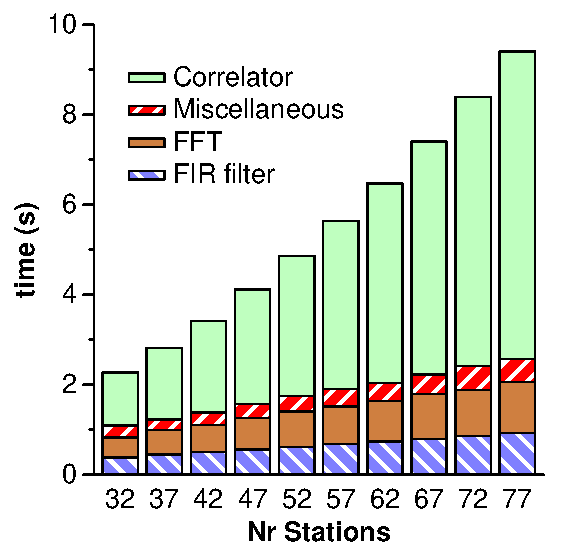
\includegraphics[width=53mm]{speed.eps}
\end{center}
\caption{Execution times of the filters for different numbers of stations}.
\label{fig:speed}
\end{figure}

After the phase correction, the data are correlated, by multiplying the
samples of each station with the complex conjugate of all other stations.
To reduce the output data rate, the correlations are typically integrated
over one second.
Since the cross correlation of station $A$ and $B$ is the complex conjugate
of station $B$ and $A$, we compute it only once.
Autocorrelations are computed as well, but treated separately since they
require only half the amount of computations.
The computational requirements of the correlator are squared in the number
of stations, and dominate the total online processing demands (see
Figure~\ref{fig:speed}).
The correlator, which is also implemented in assembly, is extremely efficient:
it achieves 98\% of the floating-point peak performance~\cite{Romein:06}.

\fixme{Storage section}


The PPF implicitly converts the 16-bit complex number to 32-bit floating-point
numbers, since the BG/L performs floating point computations faster than
integer operations.
Also, the phase correction and the correlations are done in floating point.
Internally, the BG/L only supports double-precision arithmetic, but the
high precision is not necessary for our application.



\ldots

\fixme{Maybe this paragraph should be moved to the IEEE Computer paper.}
An example that illustrates the benefits of a flexible software solution was
the ease with which we could move the second-stage PolyPhase Filter, which was
originally designed to run on FPGAs at the stations, to the Blue Gene/L.
Once we saw that we could obtain really high performance from the BG/L in
practice and recognized that sufficient computational power was left,
a considerable cost reduction was achieved by removing the PPF FPGAs from the
station design.

\ldots

Although the BG/L is computationally very efficient,
streaming the station data into the machine at the required data rates
turned out to be a major problem,
despite the BG/L's atypical high number of I/O interfaces.
For each 16~BG/L compute cores, there is one {\em I/O~node\/} that
has one external gigabit-Ethernet interface and transparently handles all I/O
calls initiated by its associated compute cores (see Figure~\ref{fig:IOnode}).
We found that the stock network system software was not particularly optimized
for high-throughput I/O, and that the obtained bandwidths were far from what
theoretically should be achievable.

The dissatisfaction about the performance and about the I/O model in general
led to a joint effort to redesign the entire network software infrastructure,
and resulted in a new environment called {\em ZOID\/}~\cite{Iskra:08}.
ZOID does not only yield better performance, but it is much more flexible,
since it allows application code to be run on the I/O~node.
With ZOID, we were able to move the receipt of the station data from the input
cluster nodes to the BG/L I/O~nodes, so that the station data are sent
directly through the WAN into the BG/L.
Not having to build a separate input cluster results in an estimated cost
saving of \euro700,000.

\section{Central Processing: Calibration}

The off-line processing of LOFAR data has to deal with a number of challenges~\cite{Noordam:04,Nijboer:07}. First of all, the data volumes are huge and being able to process the data in finite time dictates the design of the data processing chain. Second, compared to traditional steel dishes, the phased array station beams are far more variable (in time, in frequency, as well as over the different stations), they yield a higher degree of instrumental polarization, and they have relatively high sidelobes. All these issues complicate the processing of the data. Especially, since a high dynamic range must be reached. 

The third category of challenges lies in the sky itself. At the low frequencies where LOFAR will observe there will be very bright sources so that a high dynamic range and, hence, a high accuracy is needed to see the faint background sources. The sky will also be filled with a large number of sources, giving rise to confusion. Last, but not least, the Earths ionosphere seriously defocusses the images.

An introduction to signal processing for radio astronomical arrays can be found in~\cite{Veen1:04,Veen2:04,Boonstra:05}. With LOFAR we enter a new regime in radio astronomical data processing.  The challenges imply that for LOFAR we have to reconsider exisiting processing strategies and algorithms and develop new strategies and algorithms. The off-line processing therefore remains a work in progress of which we give an overview of the current status.
\label{sec:offline}

\subsection{Processing large data volumes}

The total amount of data that is produced is detemined by the total number of stations that are used in the observation. This number is still uncertain and will be different in the Low Band and the High Band, since the High Band stations in the Core will be split in 2 half stations. Using 20 Core stations and 20 Remote stations as a working example the correlator generates between 0.28 Gbyte/s for the LBA Core Array in 200 MHz sampling mode and 3.1 Gbyte/s for the HBA Full Array in 160 MHz sampling mode. After a typical observation of 4 hours between 3.3 Tbyte and 35 Tbyte will be collected, again depending on the exact mode of operation.

Since a permanent data storage is not part of the LOFAR telescope these data volumes have to be processed near real time. Fortunately, the non-imaging LOFAR applications are not so data intense, so that for every 1 hour of observation we may have up to, say, 4 hours to further process the data. With this in mind data I/O becomes a serious problem. Obviously the data needs to be processed in a parallelized and distributed way minimizing the I/O that is needed~\cite{Loose:08,Diepen:08}.  
 
Data can be distributed over a large number of processing nodes in a number of ways. Distribution over baselines is not very suitable for imaging, where data from all baselines must be combined to produce an image. Distribution over time has the disadvantage that up to sevaral Gbytes/s have to be sent to a single processing node. Frequency, therefore, seems to be the best way. This distribution scheme matches with the design of the correlator. It is also a convenient scheme for the imager, where images are created per (combined) frequency channel. 

A consequence of distribution over frequency is that in the self-calibration step solver equations from different compute nodes may need to be combined. The combining of solver equations, however, involves far less data then the underlying observed visibility data.   

Even though the processing of the data will be done on a large cluster of computers, the total amount of data can be such that we expect the quality of the final result to be processing limited. This means that for all the algorithms we have to weight accuracy against the amount of Flops needed. It also means that the LOFAR instrument can be improved by upgrading the processing cluster in the future. 

\subsection{Processing steps}

LOFAR calibration is a joint estimation problem for both instrumental parameters and source parameters. At its heart lies the ``Measurement Equation'' that is used to model the observed data~\cite{Hamaker:96}. A signal processing data model and a Cramer-Rao lower bound analysis are given in ~\cite{Tol:07}. The latter paper also provides a good introduction to the signal processing aspects of LOFAR Self-Calibration.   

The final LOFAR calibration strategy is still under development. However, we foresee that the following steps and iterations will be part of it. The first step consists of removing bad data points, which are due to e.g. Radio Frequency Interference (RFI). After this step the contaminating contribution of a couple of very strong sources (like CasA, CygA, TauA, VirA) that enter through the station beam sidelobes needs to be removed. Since modelling the station beam sidelobes is infeasible due to the large number of parameters involved, the combined effect of the sources and the instrumental effects has to be estimated and subtracted from the data. 

Once the interfering signals are removed from the data, the data may be further integrated. The high resolution in frequency is only needed for removing RFI. The final resolution is determined by bandwidth smearing requirements~\cite{SIRAII:99}. In the frequency direction the data may be reduced by a factor of 3 to 10, depending on the size of the array used for the observation {\bf CHECK}. In principle the data may also be integrated along the time axis. Here, however, we have to make sure that the effect of the ionosphere remains constant over a time sample. The maximal reduction factor determined by time-average smearing ranges from 3 tot 10, again depending on array size {\bf CHECK}.

Next an iterative loop, dubbed the ``Major Cycle'', is entered where we first estimate instrumental and source parameters using the visibility data, then image the data, and finally refine the estimation  of the source parameters using image data. Since not all parameters are estimated jointly, the Major Cycle will be traversed a number of times~\cite{Nijboer:07}. 

After initial operation of the LOFAR instrument the parameters for the strongest sources will be known. From then on the strongest sources can be used in every observation to estimate ionospheric parameters, instrumental parameters, and to refine the estimate for the station beams that is available from the station calibration. 

In~\cite{Tol:07} it is shown that the unconstrained direction dependent calibration problem is ambiguous. The authors, however, present three physical contraints to get an unambigous solution: 
%
\begin{enumerate}
\item use a calibrated subarray to calibrate the rest of the array,
\item use assumptions on the structural dependence of a certain corrupting effect, e.g. the ionosphere,
\item use polynomial smoothing on larger time / frequency domains.
\end{enumerate}
% 

In the first approach the LOFAR core is calibrated first, where use is made of the fact that the core stations all share the same ionosphere. This is a simpleer problem. Van der Tol et al. show that in this case the remote stations can be calibrated, provided the number of calibration sources is less then the number of core stations~\cite{Tol:07,Tol:05}. 

In the second approach, use is made of the fact that the effect of the ionosphere has a predictable frequency dependence~\cite{Tol:05}. The number of parameters that need to be estimated may be further reduced by using suitable base functions for the spatial dependence of the ionosphere. The use of Karhunen-Loeve base functions seems very promosing in this respect~\cite{Tol2:07}.  

In the third approach, multiple samples iin frequency and time are combined in a joint estimation, where the time and frequency dependence is modelled by e.g. polynomials and in this way the number of parameters that need to be estimated is reduced from 1 per individual sample to the polynomial coefficients for all samples together. In~\cite{Tol:07} it is reported however that this approach needs good initial estimates, since the continuous phase polynomial is ambiguous to integer multiples of $2\pi$.

For LOFAR all three approaches will used and they will be combined with the so-called ``Peeling'' approach~\cite{Noordam:04,Tol:07}.

\ldots {\bf Peeling} \ldots

The sky image is the Fourier transform of the visibility domain. Due to the fact that the visibility domain is only discretely sampled, sources in the sky image are convolved with a Point Spread Function (PSF). The contribution from sources that generate PSF far sidelobes that are higher than the image noise level should be subtracted from the visibility data. Using the solutions to the parameter estimation problem on the visibility data the contributions from the strongest sources are removed from the visibility data. The remaining residual visibility data is then corrected and imaged.

One visibility sample is the summation of contributions from all sources in the sky. Since LOFAR has a large Field of View (FoV), the contribution from different sources is distorted by different ionospheric and beam effects. When imaging the visibility data, however, it is only possible to correct the data for one direction in the sky. This would mean that the image would be sharp for the direction of correction and the image quality would degrade outwards. To overcome this problem LOFAR images will be made in facets, where we can correct the data for the center of each facet. 

Facet imaging is a well known technique to overcome the problem related to the so-called ``w-term'', which are due to the fact that the baselines are non-coplanar~\cite{SIRAII:99}. However, the non-coplanar baseline problem is better solved by the w-projection algorithm~\cite{Cornwell:05}. Therefore, we will apply the w-projection technique per facet and the facet size will only be determined by the variability of the station beam and the ionosphere.

Since we correct the data per facet, this means multiplying the total amount of data with the number of facets. Fortunately, the facet size will be far smaller then the total FoV. This allows us to shift the data to the center of the facet and then integrate the data in both time and frequency. Hence, the total amount of data will be more or less the same.
  
Once the image is produced, source finding and extraction algorithms may be used to estimate source parameters. This would then lead to an updated source model and we are ready to enter a new cycle of the Major Cycle. 

By sampling the data in each iteration of the Major Cycle, doubling the sampling density in every cycle, and using only the full resolution data in the last cycle, we effectively have not more then twice the I/O that is needed for the full resolution data. We expect that will seriously inprove the total speed of the processing.

%The correlator produces visibility data on a 1 second and 0.62 kHz of 0.78 kHz resolution depending on the sampling frequency of the station processing. The frequency resolution is needed for excision of RFI signals. Strong RFI sources can in principle be suppressed on the station level by applying spatial filtering techniques~\cite{Veen1:04,Veen2:04,Boonstra:05}. However, applying these techniques on the station level would imply that all station beams will be different. That would mean that the number of station beam parameters to be estimated in the following self-calibration step would increase considerably. We foresee that this will be impractible in the initial LOFAR operations. However, in later upgrades these spatial filtering techniques may be incorporated. Initially, LOFAR processing will use traditional flagging techniques~\cite{Renting:07}.  

\section{Current state and roll-out planning}

Currently~\cite{gunst:06}, four partially-built stations are functional: 3~stations with
16~LBAs and 1~station with 48~LBAs.
To create more baselines and achieve better UV coverage, the stations each can be split into four {\em microstations}.
This yields 16~microstations, which are treated the same as real stations in
the online and offline processing pipelines.

A consequence of quadrupling the number of stations is that the bandwidth
is reduced to 36~subbands of 195~KHz or 48~subbands of 156~KHz.
Alternatively, the station with 48~LBA can be split into 12~microstations,
so that together with the other $3\times4$ microstations a total of
24~microstations can be formed,
but WAN restrictions limit the bandwidth to 12~resp.\ 16~subbands.

\begin{figure*}
\centering
\includegraphics[width=0.32\textwidth]{LBA_observed.eps}
\includegraphics[width=0.32\textwidth]{LBA_calibrated.eps}
\includegraphics[width=0.32\textwidth]{LBA_peeled.eps}
\caption{Images from the LOFAR CS1 configuration using 48 hours and about 20 subbands of data. Observed: an image of the flagged, non-calibrated data. Calibrated: an image of the flagged, calibrated data showing CasA and CygA. Residual: an image of the flagged, calibrated data where CasA and CygA are removed from the data. Images courtesy of S.B. Yatawatta.}
\label{fig:skymap}
\end{figure*}

Figure \ref{fig:skymap} shows a series of images there were made from data using the LOFAR CS1 configuration. 16 microstations, each consisting of a single dipole with essentially an all sky FoV, were used. The images are centered on the North Celestial Pole and contain 48 hours and about 20 subbands of data. First the data is flagged for RFI and an image of the flagged-only data is shown on the left (``observed''). 

The following calibration is performed in two steps. In the first step, a point source model is used for both CasA and CygA, both at 20000 Jy flux and no polarization. An analytical beam shape is used and we solve for a single complex gain for the whole sky. In this way an estimate for the instrumental complex gains (due to e.g. clock drifts) and ionospheric phase differences is obtained. After correcting the data a second step is performed, where we estimate a complex gain in both the direction of CasA and CygA. In this second step no assumptions on the beam are made. For the middle image (``calibrated'') the data is corrected using the estimates for the direction of CasA. In this middle image CasA and CygA can be clearly seen as point sources. 

CasA and CygA completely overshine the background sources, since they are at least 50 times stronger then the average background source. After subtracting the contributions from CasA and CygA from the data the other sources become visible. This is shown in the right panel (``residual''), where now some hundred other sources are visible. 

The HBA units are currently being commissioned.
A full LBA station in Effelsberg, Germany is also operational, and will soon
be connected via a dedicated wide-area link to the Central Processor.

In the course of this year 18 full stations (13~core + 5~remote) will be produced and installed in the field. Also the WAN infrastructure and Central Processor facility will be ready in the end of 2008 to handle the data of the 18 full stations and a couple of international stations as well. In the year thereafter another 18 stations will be produced and installed in the field.

Construction of the full stations is planned as follows.
\fixme{"station" should be consistent with HBA-core "double station"}
The first 18 full stations (13~core + 5~remote) \fixme{to be confirmed}
including the WAN links to the Central Processor will be operational by the
end of 2008, and the remaining 18~stations will be built in the course of 2009.
Meanwhile, construction of international stations will continue.
The Blue Gene/L is capable of handling all foreseen future data rates.



\section{Conclusion}
The conclusion goes here.





% if have a single appendix:
%\appendix[Proof of the Zonklar Equations]
% or
%\appendix  % for no appendix heading
% do not use \section anymore after \appendix, only \section*
% is possibly needed

% use appendices with more than one appendix
% then use \section to start each appendix
% you must declare a \section before using any
% \subsection or using \label (\appendices by itself
% starts a section numbered zero.)
%


%\appendices
%\section{Proof of the First Zonklar Equation}
%Appendix one text goes here.

% you can choose not to have a title for an appendix
% if you want by leaving the argument blank
\section{}
%Appendix two text goes here.


% use section* for acknowledgement
\section*{Acknowledgment}


The authors would like to thank the LOFAR team. ASTRON is a NWO institute.

LOFAR is funded by the Dutch government in the BSIK programme for
interdisciplinary research for improvements of the knowledge infrastructure.
Additional funding is provided by the European Union, European Regional
Development Fund (EFRO) and by the ``Samenwerkingsverband Noord-Nederland,''
EZ/KOMPAS.

% Can use something like this to put references on a page
% by themselves when using endfloat and the captionsoff option.
\ifCLASSOPTIONcaptionsoff
  \newpage
\fi



% trigger a \newpage just before the given reference
% number - used to balance the columns on the last page
% adjust value as needed - may need to be readjusted if
% the document is modified later
%\IEEEtriggeratref{8}
% The "triggered" command can be changed if desired:
%\IEEEtriggercmd{\enlargethispage{-5in}}

% references section

% can use a bibliography generated by BibTeX as a .bbl file
% BibTeX documentation can be easily obtained at:
% http://www.ctan.org/tex-archive/biblio/bibtex/contrib/doc/
% The IEEEtran BibTeX style support page is at:
% http://www.michaelshell.org/tex/ieeetran/bibtex/
%\bibliographystyle{IEEEtran}
% argument is your BibTeX string definitions and bibliography database(s)
%\bibliography{IEEEabrv,../bib/paper}
%
% <OR> manually copy in the resultant .bbl file
% set second argument of \begin to the number of references
% (used to reserve space for the reference number labels box)
%\begin{thebibliography}{1}
%
%\bibitem{IEEEhowto:kopka}
%H.~Kopka and P.~W. Daly, \emph{A Guide to \LaTeX}, 3rd~ed.\hskip 1em plus
%  0.5em minus 0.4em\relax Harlow, England: Addison-Wesley, 1999.
%
%\end{thebibliography}
\bibliographystyle{IEEEtran}
\bibliography{lofar,lofarRJN}

% biography section
% 
% If you have an EPS/PDF photo (graphicx package needed) extra braces are
% needed around the contents of the optional argument to biography to prevent
% the LaTeX parser from getting confused when it sees the complicated
% \includegraphics command within an optional argument. (You could create
% your own custom macro containing the \includegraphics command to make things
% simpler here.)
%\begin{biography}[{\includegraphics[width=1in,height=1.25in,clip,keepaspectratio]{mshell}}]{Michael Shell}
% or if you just want to reserve a space for a photo:

\begin{IEEEbiography}{Andr\'{e} W. Gunst}
Biography text here.
\end{IEEEbiography}

\begin{IEEEbiography}[{\includegraphics[width=1in,height=1.25in,clip,keepaspectratio]{rnijboer.eps}}]{Ronald Nijboer}
Blah blah blah.
\end{IEEEbiography}


% if you will not have a photo at all:
%\begin{IEEEbiographynophoto}{John Doe}
%Biography text here.
%\end{IEEEbiographynophoto}

% insert where needed to balance the two columns on the last page with
% biographies
%\newpage

\begin{IEEEbiographynophoto}{John W. Romein}
Biography text here.
\end{IEEEbiographynophoto}

% You can push biographies down or up by placing
% a \vfill before or after them. The appropriate
% use of \vfill depends on what kind of text is
% on the last page and whether or not the columns
% are being equalized.

%\vfill

% Can be used to pull up biographies so that the bottom of the last one
% is flush with the other column.
%\enlargethispage{-5in}



% that's all folks
\end{document}


